%%%%%%%%%%%%%%%%%%%%%%%%%%%%%%%%%%%%%%%%%
% a0poster Portrait Poster
% LaTeX Template
% Version 1.0 (22/06/13)
%
% The a0poster class was created by:
% Gerlinde Kettl and Matthias Weiser (tex@kettl.de)
%
% This template has been downloaded from:
% http://www.LaTeXTemplates.com
%
% License:
% CC BY-NC-SA 3.0 (http://creativecommons.org/licenses/by-nc-sa/3.0/)
%
%%%%%%%%%%%%%%%%%%%%%%%%%%%%%%%%%%%%%%%%%

%----------------------------------------------------------------------------------------
%	PACKAGES AND OTHER DOCUMENT CONFIGURATIONS
%----------------------------------------------------------------------------------------

\documentclass[a0,portrait]{a0poster}

\usepackage{multicol} % This is so we can have multiple columns of text side-by-side
\columnsep=100pt % This is the amount of white space between the columns in the poster
\columnseprule=3pt % This is the thickness of the black line between the columns in the poster

\usepackage[svgnames]{xcolor} % Specify colors by their 'svgnames', for a full list of all colors available see here: http://www.latextemplates.com/svgnames-colors

\usepackage{times} % Use the times font
%\usepackage{palatino} % Uncomment to use the Palatino font

\usepackage{graphicx} % Required for including images
\graphicspath{{figures/}} % Location of the graphics files
\usepackage{booktabs} % Top and bottom rules for table
\usepackage[font=small,labelfont=bf]{caption} % Required for specifying captions to tables and figures
\usepackage{amsfonts, amsmath, amsthm, amssymb} % For math fonts, symbols and environments
\usepackage{wrapfig} % Allows wrapping text around tables and figures

%% MY CODE
\usepackage{float}
\usepackage{array}
\usepackage{amsmath}
%\usepackage{biblatex}
\usepackage{tikz}
\usepackage{enumitem}
\usepackage[hidelinks]{hyperref}

\usetikzlibrary{positioning, shadows, arrows.meta, shapes}
\setlist[itemize]{noitemsep, topsep=0pt}
\setlist[enumerate]{noitemsep, topsep=0pt}

% Load polyglossia for multilingual support
\usepackage{polyglossia}
\setmainlanguage{english}
\setotherlanguage{russian}

\captionsetup[table]{skip=5pt}
\captionsetup[figure]{skip=5pt}


\usepackage{titlesec}
% Syntax: \titlespacing*{<command>}{<left>}{<before-sep>}{<after-sep>}
\titlespacing*{\section}{0pt}{1.5ex plus 1ex minus 0.2ex}{0.5ex plus 0.2ex}
\titlespacing*{\subsection}{0pt}{1.25ex plus 0.5ex minus 0.2ex}{0.3ex plus 0.2ex}
\titlespacing*{\subsubsection}{0pt}{1ex plus 0.3ex minus 0.2ex}{0.1ex plus 0.2ex}

% Choose a main font that supports Cyrillic
\setmainfont{Times New Roman} % Replace with a font available on your system
%%

\begin{document}

%----------------------------------------------------------------------------------------
%	POSTER HEADER
%----------------------------------------------------------------------------------------

% The header is divided into two boxes:
% The first is 75% wide and houses the title, subtitle, names, university/organization and contact information
% The second is 25% wide and houses a logo for your university/organization or a photo of you
% The widths of these boxes can be easily edited to accommodate your content as you see fit

\begin{minipage}[b]{0.9\linewidth}
\huge \color{NavyBlue} \textbf{Interpretable approach to detecting semantic changes based on generated definitions} \color{Black}\\[0.2cm] % Title
%\Huge\textit{An Exploration of Complexity}\\[2cm] % Subtitle
\huge \textbf{Tatarinov Maksim \& Demidovsky Aleksandr}\\[0.3cm] % Author(s)
\Large HSE University, Nizhny Novgorod\\[0.2cm] % University/organization
\Large \texttt{tatarinovst0@gmail.com, monadv@yandex.ru}
\end{minipage}
\hspace*{1cm}
%
\begin{minipage}[b]{0.1\linewidth}
\centering

\includegraphics[width=8cm]{img/frame}\\
\textbf{GitHub}
\end{minipage}

%\vspace{0.1cm} % A bit of extra whitespace between the header and poster content

%----------------------------------------------------------------------------------------

\begin{multicols}{2} % This is how many columns your poster will be broken into, a portrait poster is generally split into 2 columns

%----------------------------------------------------------------------------------------
%	ABSTRACT
%----------------------------------------------------------------------------------------
%
%\color{Navy} % Navy color for the abstract
%
%\begin{abstract}
%
%This paper investigates definition modeling as an approach to semantic change detection,
%which offers the advantage of providing human-readable explanations, unlike traditional embedding-based approaches that lack interpretability.
%Definition modeling leverages large language models to generate dictionary-like definitions based on target words and their contextual usages.
%Despite its potential, practical evaluations of this method remain scarce.
%In this study, FRED-T5 was fine-tuned using the Small Academic Dictionary for the task of definition modeling.
%Both quantitative and qualitative assessments of definition modeling's effectiveness in detecting semantic shifts within the Russian language were conducted.
%The approach achieved a Spearman's rank correlation coefficient of 0.815 on the Rushifteval task, demonstrating strong alignment with expert annotations and ranking among the leading solutions.
%For interpretability, a visualization algorithm was proposed that displays semantic changes over time.
%In the qualitative evaluation, our system successfully replicated manual linguistic analysis of 20 Russian words that had undergone semantic shifts.
%Analysis of the generated meanings and their temporal frequencies showed that this approach could be valuable for historical linguists and lexicographers.
%
%\end{abstract}

%----------------------------------------------------------------------------------------
%	INTRODUCTION
%----------------------------------------------------------------------------------------

\color{SaddleBrown} % SaddleBrown color for the introduction

\section*{Introduction}

Static and contextual embeddings excel at capturing semantic relationships for detecting semantic change,
but lack human-readable word descriptions.
Advancements in recent research involve definition generation with language models, which offer more illustrative descriptions~\cite{DefinitionGenerationMainArticle,fedorova-etal-2024-definition}.
It could aid historical linguists and lexicographers in creating dictionaries and language history studies, such as \newcite{TwoCenturies}.
However, the practical evaluation of this approach remains limited.

The primary \textbf{objective} of this study is to \textbf{assess the effectiveness of language models in detecting semantic changes in words through the generation of definitions}.
It would include:
\begin{itemize}
    \item \textbf{quantitative metrics from a shared task};
    \item \textbf{qualitative analysis by reproducing a linguistic analysis of words known to have undergone semantic shifts}.
\end{itemize}

%\color{DarkSlateGray} % DarkSlateGray color for the rest of the content
\color{Black}

%----------------------------------------------------------------------------------------
%	MATERIALS AND METHODS
%----------------------------------------------------------------------------------------

\section*{Definition Modeling}

\begin{center}
\begin{tikzpicture}[
    box/.style={
        rectangle,
        rounded corners,
        draw,
        drop shadow,
        fill=#1!20,
        text width=10cm,
        align=center,
        minimum height=4em
    },
    box-small/.style={
        rectangle,
        rounded corners,
        draw,
        drop shadow,
        fill=#1!20,
        text width=3.5cm,
        align=center,
        minimum height=4em
    },
    arrow/.style={
        thick,
        -{Stealth[scale=1.2]},
        draw=#1
    },
    label/.style={
        font=\footnotesize
    }
]

    % Define Colors
    \definecolor{inputcolor}{RGB}{135,206,250}    % Light Sky Blue
    \definecolor{modelcolor}{RGB}{144,238,144}    % Light Green
    \definecolor{outputcolor}{RGB}{255,182,193}   % Light Pink

    % Nodes
    \node[box=inputcolor] (input) {
        \textbf{Example usage} \\
        He started to sleep poorly at night, waking up with a persistent headache. \\
        \textbf{Target word: \textit{night}}
    };

    \node[box-small=modelcolor, right=4cm of input] (llm) {  % Use box-small style here
        \textbf{Large\\Language\\Model}
    };

    \node[box=outputcolor, right=4cm of llm] (output) {
        \textbf{Generated definition} \\
        The part of the day from sunset to sunrise.
    };

    % Arrows with Labels Positioned Above
    \draw[arrow=black] (input) -- node[midway, above] {Input} (llm);
    \draw[arrow=black] (llm) -- node[midway, above] {Output} (output);

\end{tikzpicture}
\end{center}

\section*{Model and Data}

FRED-T5-1.7B was chosen due to its performance in processing Russian~\cite{FRED-T5}.
At the time of selection, it was the top performer on the RussianSuperGLUE benchmark~\cite{RussianSuperGLUE}, with a score of 0.762.

FRED-T5-1.7B was trained with the task of generating an accurate definition on a dataset
where each entry contained a word, its context, and a corresponding definition.
%The model learned to generate an accurate definition by minimizing the cross-entropy loss between its predicted token probabilities and the reference definitions:
%Data extraction was performed using a Python-based scraper.

\subsubsection*{Data}
The training dataset was based on \("\)Small academic dictionary\("\)~\cite{MAS1981}.
It was cleaned to:
\begin{itemize}
    \item remove usage labels;
    \item entries without usage examples;
    \item entries without informative definitions, such as \textit{Состояние по знач. глаг. линять} [\textit{State by the meaning of the verb "to shed"}];
    \item those that provided grammatical rather than lexical information, such as \textit{наречие к причастию приглашающий} [\textit{Adverb to the participle "inviting"}].
\end{itemize}
This resulted in 122,350 entries, with 90\% in the training part.
%The resulting dataset of 122,350 entries was partitioned into training, validation, and test sets with a 90/5/5 split.

%Each entry was formatted and began with the word \("\)Контекст\("\) [\("\)Context\("\)] followed by a usage example, then the phrase \("\)Определение слова\("\) [\("\)Word definition\("\)], and the word itself.\footnote{A special denoiser token \texttt{<LM>}, dedicated to the task of text continuation, was utilized.}

\section*{Shared Task Evaluation}

\subsection*{Data}

The \textit{RuShiftEval} task's test set~\cite{rushifteval} was utilized for evaluation.
The task focuses on detecting semantic changes in Russian nouns across three historical transitions:
\begin{itemize}
    \item RuShiftEval-1 (Pre-Soviet:Soviet);
    \item RuShiftEval-2 (Soviet:Post-Soviet);
    \item RuShiftEval-3 (Pre-Soviet:Post-Soviet).
\end{itemize}
The task provided a test set of gold change scores for 99 Russian nouns corresponding to the transitions.
%Evaluation was conducted using Spearman's rank correlation to measure the alignment between the approach's results and the gold scores.

\subsection*{Pipeline}

\usetikzlibrary{positioning, shadows, arrows.meta}

\begin{tikzpicture}[auto,
  node distance=2cm,  % sets a default distance between nodes
  block/.style={
      rectangle,
      draw,
      rounded corners,
      minimum width=3.5cm,
      minimum height=1.2cm,
      align=center,
      drop shadow},
  arrow/.style={-{Stealth[scale=1.2]}, thick}
]

\node[block, fill=red!20] (sampling)
    {Sampling 100 usages for each of 99 test words\\per period from diachronic sub-corpus\\of the Russian National Corpus};

\node[block, fill=green!20, below=of sampling] (pairing)
    {Pairing of usages\\across period transitions};

\node[block, fill=orange!20, below=of pairing] (defgen)
    {Definition\\generation};


\node[block, fill=purple!20, right=4.6cm of sampling] (vectorize)
    {Vectorization};

\node[block, fill=yellow!20, below=of vectorize] (cosine)
    {Cosine distance\\calculation};

\node[block, fill=teal!20, below=of cosine] (evaluation)
    {Comparing mean scores\\with gold scores\\using Spearman's rank correlation};

\draw[arrow] (sampling) -- node[midway, left] {Word usages} (pairing);
\draw[arrow] (pairing) -- node[midway, left] {\parbox{10cm}{100 pairs of usages\\per transition for each word}} (defgen);
\draw[arrow] (defgen.east) to[out=0, in=180] node[sloped, midway, below] {Generated definitions} (vectorize.west);

\draw[arrow] (vectorize) -- node[midway, right] {Vector representations} (cosine);
\draw[arrow] (cosine) -- node[midway, right] {Semantic similarity scores} (evaluation);

\end{tikzpicture}

\subsection*{Results}

%Our approach to solving the task is similar to \newcite{DeepMistake} and involves reproducing the RuShiftEval annotation effort.
%For 99 test words from the Rushifteval competition, 100 sentences (or all, if there were fewer) were randomly sampled for each period from the diachronic sub-corpus of the Russian National Corpus~\cite{Ruscorpora}.
%For each period transition, the usages were paired, and the model generated definitions for each pair.
The paraphrase-multilingual-mpnet-base-v2 model~\cite{Vectorizer}, additionally fine-tuned on RuSemShift, a similar dataset~\cite{rusemshift}, was used to vectorize definitions.
%The distances between the definitions were calculated using the cosine distance.
%After that, mean values of the ratings for each word were compared with the gold scores using Spearman's rank correlation.

\begin{table}[H]
\centering
\begin{tabular}{|m{12cm}|m{4.5cm}|m{9cm}|m{6cm}|}
\hline
\textbf{Team} & \textbf{Average} & \textbf{Word Representation Type} & \textbf{Model Used} \\
\hline
\textbf{DeepMistake (post-competition)} & \textbf{0.850} & \textbf{Contextual Emb.} & \textbf{XLM-R} \\
\hline
\textbf{Proposed Approach} & \textbf{0.815} & \textbf{Generated Definitions} & \textbf{FRED-T5-1.7B} \\
\hline
GlossReader & 0.802 & Contextual Emb. & XLM-R \\
\hline
DeepMistake & 0.791 & Contextual Emb. & XLM-R \\
\hline
Other 11 Teams & 0.720-0.178 & \ldots & \ldots \\
\hline
\end{tabular}
\caption{Algorithm Results Compared to RuShiftEval Teams}
\label{tab:Rushifteval_all}
\end{table}

The proposed approach outperforms most entries in the RuShiftEval task, as shown in Table~\ref{tab:Rushifteval_all}.

\begin{table}[H]
\centering
\begin{tabular}{|m{8cm}|m{5.5cm}|m{5.5cm}|m{5.5cm}|m{5cm}|}
\hline
\textbf{Method} & \textbf{RuShiftEval-1} & \textbf{RuShiftEval-2} & \textbf{RuShiftEval-3} & \textbf{Base Model} \\
\hline
\textbf{Proposed Approach without vectorizer fine-tuning} & \textbf{0.722} & \textbf{0.763} & \textbf{0.749} & \textbf{FRED-T5-1.7B} \\
\hline
\newcite{fedorova-etal-2024-definition} & 0.488 & 0.462 & 0.504 & MT0-XL \\
\hline
\end{tabular}
\caption{Comparison with Definition Generation Approaches}
\label{tab:Definition_modeling_results}
\end{table}

A shown in Table~\ref{tab:Definition_modeling_results},
the proposed approach significantly outperforms the results of \newcite{fedorova-etal-2024-definition}.
The vectorizer fine-tuning step was omitted to ensure compatability of the results.%that the results are directly comparable.

\newcite{fedorova-etal-2024-definition} appears to retain unhelpful definitions in the training data, possibly resulting in their model reproducing non-informative patterns and the lower performance of their approach.

\section*{Qualitative Evaluation}

20 words exhibiting shifts from \textit{Two Centuries in Twenty Words}~\cite{TwoCenturies} are selected:
\textit{знатный [noble]}, \textit{кануть [to disappear]}, \textit{классный [classy/cool]}, \textit{мама [mom]}, \textit{машина [machine/car]},
\textit{молодец [young man/attaboy]}, \textit{пакет [bag/package]}, \textit{передовой [advanced]}, \textit{пионер [pioneer]},
\textit{пожалуй [perhaps]}, \textit{пока [until/bye]}, \textit{привет [hello]}, \textit{пружина [spring]}, \textit{публика [public]},
\textit{свалка [landfill/fight]}, \textit{сволочь [bastard]}, \textit{стиль [style]},
\textit{тётка [aunt]}, \textit{тройка [three/a set of three]}, \textit{червяк [worm]}.
300 usage examples per word per period are obtained from the diachronic sub-corpus of Russian National Corpus~\cite{Ruscorpora}.
The trained model generates definitions for each word usage.
To obtain meanings and changes in their usages, a visualization algorithm is applied.
The definitions from the visualization are compared with information from semantic descriptions of words,
written based on \newcite{SemanticDefinitionsAndAnalysis} method of generalizing multiple dictionary definitions,
and classified according to the error types.
Finally, changes in the frequency of meanings over time provided by the visualizations are compared with historical data from \textit{Two Centuries in Twenty Words}.

\subsection*{Visualization}

Generated definitions are transformed into vector representations using a vectorizer and clustered using DBSCAN.
Each cluster is represented by a prototypical definition closest to its centroid.
%DBSCAN parameters (\texttt{eps} and \texttt{min\_samples}) are manually tuned by incremental adjustment to ensure the formation of cohesive clusters.
%as there is no predefined optimal method for clustering semantically similar definitions.
%Then, the temporal distribution of these meanings is displayed using bar charts, as shown in Figure~\ref{fig:Машина_example}.

\begin{figure}[H]
    \centering
    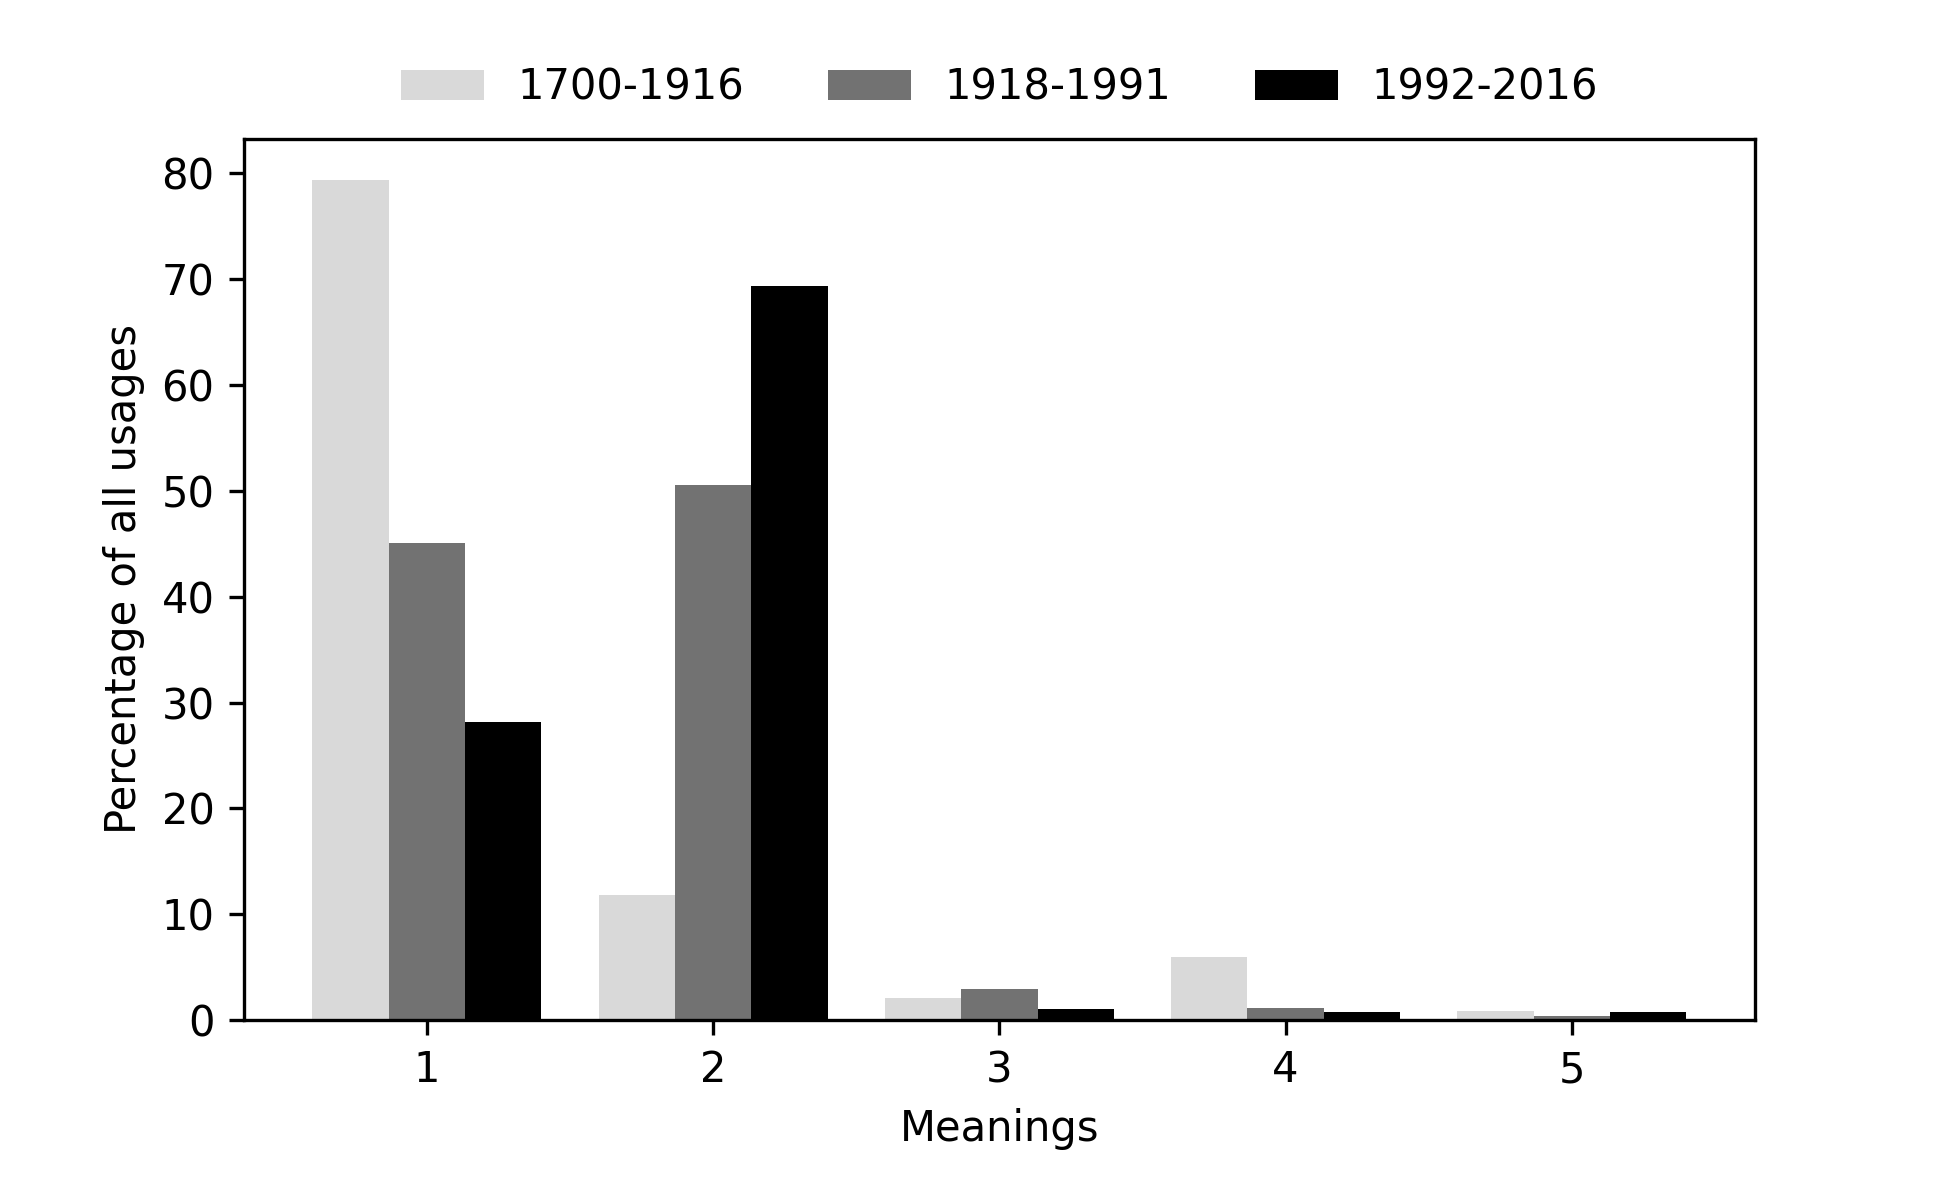
\includegraphics[width=0.3\textwidth]{img/mashina_minimal}
    \caption{Semantic Shift of the Word \textit{машина [machine/car]} (Parameters: eps=0.14, min\_samples=5)}
    \label{fig:Машина_example}
\end{figure}

\begin{center}
    \begin{minipage}{0.4\textwidth}
        \centering
        \textbf{Meanings for \textit{машина [machine/car]}:}\\
        \begin{enumerate}[leftmargin=7cm]
            \item A device or instrument for a specific task.
            \item An automobile or vehicle.
            \item An aircraft or helicopter.
            \item A mechanically or thoughtlessly acting person.
            \item A system, a collection of institutions or organizations.
        \end{enumerate}
    \end{minipage}
\end{center}

%------------------------------------------------

%\subsection*{Mathematical Section}
%
%Nulla vel nisl sed mauris auctor mollis non sed.
%
%\begin{equation}
%E = mc^{2}
%\label{eqn:Einstein}
%\end{equation}
%
%Curabitur mi sem, pulvinar quis aliquam rutrum. (1) edf (2)
%, $\Omega=[-1,1]^3$, maecenas leo est, ornare at. $z=-1$ edf $z=1$ sed interdum felis dapibus sem. $x$ set $y$ ytruem.
%Turpis $j$ amet accumsan enim $y$-lacina;
%ref $k$-viverra nec porttitor $x$-lacina.
%
%Vestibulum ac diam a odio tempus congue. Vivamus id enim nisi:
%
%\begin{eqnarray}
%\cos\bar{\phi}_k Q_{j,k+1,t} + Q_{j,k+1,x}+\frac{\sin^2\bar{\phi}_k}{T\cos\bar{\phi}_k} Q_{j,k+1} &=&\nonumber\\
%-\cos\phi_k Q_{j,k,t} + Q_{j,k,x}-\frac{\sin^2\phi_k}{T\cos\phi_k} Q_{j,k}\label{edgek}
%\end{eqnarray}
%and
%\begin{eqnarray}
%\cos\bar{\phi}_j Q_{j+1,k,t} + Q_{j+1,k,y}+\frac{\sin^2\bar{\phi}_j}{T\cos\bar{\phi}_j} Q_{j+1,k}&=&\nonumber \\
%-\cos\phi_j Q_{j,k,t} + Q_{j,k,y}-\frac{\sin^2\phi_j}{T\cos\phi_j} Q_{j,k}.\label{edgej}
%\end{eqnarray}
%
%Nulla sed arcu arcu. Duis et ante gravida orci venenatis tincidunt. Fusce vitae lacinia metus. Pellentesque habitant morbi. $\mathbf{A}\underline{\xi}=\underline{\beta}$ Vim $\underline{\xi}$ enum nidi $3(P+2)^{2}$ lacina. Id feugain $\mathbf{A}$ nun quis; magno.

%----------------------------------------------------------------------------------------
%	RESULTS
%----------------------------------------------------------------------------------------

\subsection*{Results}

As a result of generalizing dictionary definitions, 121 meanings were compiled for 20 words.
83 definitions were obtained using the proposed approach.
Thus, excluding 5 incorrect definitions, out of 121 meanings 64.4\% were identified.

\begin{table}[H]
\centering
\label{tab:definitions_classification}
\begin{tabular}{|>{\raggedright\arraybackslash}p{20cm}|c|c|}
\hline
\textbf{Type of Definition} & \textbf{Count} & \textbf{Percentage} \\ \hline
Correct & 57 & 68.67\% \\ \hline
Close & 10 & 12.04\% \\ \hline
Incorrect & 5 & 6.02\% \\ \hline
Redundancy or Excessive Use of General Phrases & 4 & 4.81\% \\ \hline
Insufficiently Specific & 3 & 3.61\% \\ \hline
Overly Specific & 3 & 3.61\% \\ \hline
Close, Redundancy or Excessive Use of General Phrases & 1 & 1.20\% \\ \hline
Self-reference & 0 & 0.00\% \\ \hline
Opposite Meaning & 0 & 0.00\% \\ \hline
Incorrect Part of Speech & 0 & 0.00\% \\ \hline
\end{tabular}
\caption{Types of Definitions and Their Counts}
\end{table}

The majority of definitions are correct without any errors or shortcomings (68.67\%).

%Common issues include close or incorrect meanings, such as defining \textit{червяк [worm]} as an adult insect or describing \textit{пожалуй [perhaps]} as a conjunction.
%Redundancy is present, exemplified by the repetitive “chaotic” in the definition of \textit{свалка [landfill/fight]} (‘Беспорядочная, беспорядочная схватка’),
%possibly due to the abundance of synonymous expressions in the training dataset, a common method in lexicology.
%Additionally, some definitions lack specificity, such as describing \textit{мама [mom]} simply as ‘a tender address to a woman.’
%These problems may arise from the model's limited world knowledge.
%
%Another issue is insufficient context, leading to ambiguity in distinguishing meanings,
%as seen with \textit{пионер [pioneer]} in \textit{Pioneers listen to this and admire it [Пионеры слушают это и восхищаются].}

\begin{table}[H]
\centering
\label{tab:Statistical}
\begin{tabular}{|m{9cm}|m{6cm}|}
\hline
\textbf{Results} & \textbf{Word amount} \\
\hline
Correct & 12 \\
\hline
Partially correct & 4 \\
\hline
Incorrect & 1 \\
\hline
Full analysis not possible & 3 \\
\hline
\end{tabular}
\caption{Results of Statistical Analysis of Semantic Shifts}
\end{table}

Overall, main meaning changes consistent with the book's data were identified in 12 out of 20 words.
Additionally, changes partially aligned in 4 other words.
A full analysis is not feasible for \textit{публика [public]}, \textit{кануть [to disappear]} and \textit{сволочь [bastard]}
due to \textit{Two Centuries in Twenty Words} not having sufficient diagrams or detected meanings falling under one in the book.

%----------------------------------------------------------------------------------------
%	CONCLUSIONS
%----------------------------------------------------------------------------------------

\color{SaddleBrown} % SaddleBrown color for the conclusions to make them stand out

\section*{Conclusions}

\begin{itemize}
    \item The study demonstrated the effectiveness of definition modeling in detecting semantic shifts.% in Russian.
    \item A FRED-T5-1.7B model, fine-tuned on the \("\)Small academic dictionary\("\), was used to generate context-based word definitions.
    \item The model performed among the top solutions of RuShiftEval and outperformed \newcite{fedorova-etal-2024-definition}.
    \item A visualization algorithm was developed to represent semantic changes over time, allowing for reproducing a manual effort of studying semantic changes for a set of 20 words.
    \item Qualitative analysis revealed that 68.67\% of generated definitions were fully correct, with main changes fully detected in 12 out of 17 words available for analysis and partial alignment in 4.
\end{itemize}

\color{DarkSlateGray} % Set the color back to DarkSlateGray for the rest of the content

%----------------------------------------------------------------------------------------
%	FORTHCOMING RESEARCH
%----------------------------------------------------------------------------------------

%\section*{Forthcoming Research}
%
%Vivamus molestie, risus tempor vehicula mattis, libero arcu volutpat purus, sed blandit sem nibh eget turpis. Maecenas rutrum dui blandit lorem vulputate gravida. Praesent venenatis mi vel lorem tempor at varius diam sagittis. Nam eu leo id turpis interdum luctus a sed augue. Nam tellus.

 %----------------------------------------------------------------------------------------
%	REFERENCES
%----------------------------------------------------------------------------------------

%\nocite{*} % Print all references regardless of whether they were cited in the poster or not
%{
%%\footnotesize
%\bibliographystyle{dialogue}
%\bibliography{sample}
%}
\makeatletter
\renewcommand{\@biblabel}[1]{}
\makeatother

\begingroup
\scalebox{1.2}{% Change 2 to the necessary scale factor (the reciprocal of the poster's scale)
  \begin{minipage}{0.85\linewidth} % adjust the minipage width accordingly
    {
%\footnotesize

\bibliography{sample}
    \bibliographystyle{dialogue}
}
  \end{minipage}
}
\endgroup


%----------------------------------------------------------------------------------------
%	ACKNOWLEDGEMENTS
%----------------------------------------------------------------------------------------

%\section*{Acknowledgements}
%
%Etiam fermentum, arcu ut gravida fringilla, dolor arcu laoreet justo, ut imperdiet urna arcu a arcu. Donec nec ante a dui tempus consectetur. Cras nisi turpis, dapibus sit amet mattis sed, laoreet.

%----------------------------------------------------------------------------------------

\end{multicols}
\end{document}